\documentclass[a4paper,11pt]{article}

\usepackage[utf8]{inputenc}
\usepackage[T1]{fontenc}
\usepackage[main=ngerman,provide=*]{babel}
\usepackage{lmodern}
\usepackage{microtype}
\usepackage{geometry}
\usepackage{graphicx}
\usepackage{setspace}
\usepackage{parskip}
\usepackage{booktabs}
\usepackage{tabularx}
\usepackage{array}
\usepackage{longtable}
\usepackage{float}
\usepackage{enumitem}
\usepackage{xcolor}
\usepackage{fancyhdr}
\usepackage{titlesec}
\usepackage{tikz}
\usepackage{hyperref}

\usetikzlibrary{
  arrows.meta,
  positioning,
  shapes.geometric,
  fit,
  backgrounds,
  calc
}

\graphicspath{{images/}}

\geometry{
  left=2.7cm,
  right=2.7cm,
  top=2.6cm,
  bottom=2.6cm
}

\setstretch{1.15}
\setlength{\emergencystretch}{3em}
\setlength{\parindent}{0pt}
\setlength{\parskip}{0.55em}

\renewcommand{\arraystretch}{1.25}

\setlist[itemize]{
  topsep=0.35em,
  itemsep=0.2em,
  leftmargin=1.5em
}

\definecolor{LayerBlue}{HTML}{DCEBFA}
\definecolor{LayerGreen}{HTML}{DDF3E4}
\definecolor{LayerOrange}{HTML}{FCE8D5}
\definecolor{LayerPurple}{HTML}{E9E1F8}
\definecolor{LayerGray}{HTML}{F2F3F5}
\definecolor{DarkBlue}{HTML}{1F4E79}
\definecolor{DarkGreen}{HTML}{256D3F}
\definecolor{DarkOrange}{HTML}{9A4C00}
\definecolor{DarkPurple}{HTML}{5B3C88}

\newcolumntype{Y}{>{\raggedright\arraybackslash}X}
\newcolumntype{L}[1]{>{\raggedright\arraybackslash}p{#1}}

\titleformat{\section}[block]
  {\normalfont\bfseries\fontsize{22pt}{26pt}\selectfont}
  {\thesection}
  {0.8em}
  {}

\titlespacing*{\section}
  {0pt}
  {1.6em}
  {0.8em}

\titleformat{\subsection}[block]
  {\normalfont\bfseries\Large}
  {\thesubsection}
  {0.8em}
  {}

\titlespacing*{\subsection}
  {0pt}
  {1.2em}
  {0.5em}

\titleformat{\subsubsection}[block]
  {\normalfont\bfseries\large}
  {\thesubsubsection}
  {0.8em}
  {}

\titlespacing*{\subsubsection}
  {0pt}
  {1em}
  {0.4em}

\pagestyle{fancy}
\fancyhf{}

\fancyfoot[C]{\thepage}

\renewcommand{\headrulewidth}{0pt}
\renewcommand{\footrulewidth}{0pt}

\hypersetup{
  pdftitle={Architekturdokumentation Bewerbungstracker},
  pdfauthor={Philipp Söllner, Tom Petzold, Sascha Vusatjuk},
  colorlinks=true,
  linkcolor=black,
  citecolor=black,
  urlcolor=DarkBlue
}

\tikzset{
  box/.style={
    draw,
    rounded corners=2pt,
    thick,
    align=center,
    minimum height=1.15cm,
    text width=3.2cm
  },
  system/.style={
    box,
    fill=LayerBlue,
    draw=DarkBlue
  },
  actor/.style={
    box,
    fill=LayerGray,
    draw=black,
    text width=2.6cm
  },
  frontend/.style={
    box,
    fill=LayerPurple,
    draw=DarkPurple
  },
  backend/.style={
    box,
    fill=LayerBlue,
    draw=DarkBlue
  },
  database/.style={
    cylinder,
    shape border rotate=90,
    aspect=0.25,
    draw=DarkGreen,
    thick,
    fill=LayerGreen,
    align=center,
    minimum height=1.35cm,
    minimum width=2.9cm
  },
  filebox/.style={
    box,
    fill=LayerOrange,
    draw=DarkOrange,
    text width=2.8cm
  },
  layer/.style={
    draw,
    rounded corners=2pt,
    thick,
    minimum width=9.5cm,
    minimum height=1.25cm,
    align=center
  },
  participant/.style={
    draw,
    rounded corners=2pt,
    thick,
    fill=LayerGray,
    minimum width=2.55cm,
    minimum height=0.8cm,
    align=center
  },
  message/.style={
    -{Latex[length=2.2mm]},
    thick
  },
  return/.style={
    -{Latex[length=2.2mm]},
    dashed
  },
  connection/.style={
    -{Latex[length=2.4mm]},
    thick
  },
  state/.style={
    draw,
    rounded corners=9pt,
    thick,
    fill=LayerGray,
    minimum width=2.15cm,
    minimum height=0.8cm,
    align=center
  }
}

\begin{document}





% ================================  Deckblatt ✓ =================================

\hypersetup{pageanchor=false}

\begin{titlepage}
\thispagestyle{empty}

\begin{center}

\begin{minipage}{\textwidth}
  
\includegraphics[height=3cm]{images/rwu-logo.png}
  \hfill
  
\includegraphics[height=2cm]{images/arc42-logo.png}
\end{minipage}

\vspace{1.5cm}

{\Large\textsc{Hochschule Ravensburg-Weingarten}\par}
\vspace{0.4cm}

{\large Lehrveranstaltung Software-Architektur\par}
{\large Sommersemester 2026\par}

\vspace{0.5cm}

\rule{\textwidth}{0.5pt}

\vspace{0.5cm}

{\Huge\bfseries Architekturdokumentation\par}

\vspace{0.5cm}

{\LARGE\bfseries Bewerbungstracker\par}

\vspace{0.5cm}

{\Large Umsetzung einer Schichtenarchitektur\par}

\vspace{0.3cm}

{\large Dokumentationsstruktur nach arc42\par}

\vspace{0.6cm}

\rule{\textwidth}{0.5pt}

\end{center}

\vfill

\noindent
\begin{minipage}[t]{0.52\textwidth}
  \raggedright
  \large

  \textbf{Verfasser}\par
  \vspace{0.3cm}

  Philipp Söllner, 35601\par
  \vspace{0.2cm}

  Tom Petzold, 34917\par
  \vspace{0.2cm}

  Sascha Vusatjuk, 35650\par
\end{minipage}
\hfill
\begin{minipage}[t]{0.42\textwidth}
  \raggedright
  \large

  \textbf{Betreuer}\par
  \vspace{0.3cm}

  Prof. Dr. Sebastian Mauser\par
  Hochschule Ravensburg-Weingarten\par
\end{minipage}

\vfill

\begin{center}
  {\large Weingarten, 31. Juli 2026}
\end{center}

\end{titlepage}

\hypersetup{pageanchor=true}
\pagenumbering{roman}





% ===========================  0 Inhaltsverzeichnis ✓ ===========================

\thispagestyle{plain}
\tableofcontents
\clearpage

\pagenumbering{arabic}
\setcounter{page}{1}





% ===========================  1 Einführung und Ziele ✓ ===========================

\section{Einführung und Ziele}

\subsection{Aufgabenstellung}

Der Bewerbungstracker ist eine webbasierte Anwendung zur Verwaltung und Nachverfolgung persönlicher Bewerbungsprozesse.
Nutzer können Bewerbungen erfassen, bearbeiten und nach ihrem aktuellen Status organisieren.
Der Bewerbungsprozess wird vom Entwurf bis zu einem abschließenden Zustand abgebildet.

Die wesentlichen Funktionen sind:

\begin{itemize}
  \item Anlegen, Bearbeiten und Löschen von Bewerbungen
  \item Darstellung der Bewerbungen auf einem Kanban-Board
  \item Ändern des Status per Drag-and-drop oder Auswahlmenü
  \item Prüfung zulässiger Statusübergänge
  \item Anzeige einer Änderungshistorie
  \item Zurücksetzen der letzten Statusänderung
  \item Suche über die Bewerbungsdaten
  \item Anzeige statistischer Kennzahlen
\end{itemize}

Das Projekt dient der praktischen Umsetzung einer Layered Architecture.
Der architektonische Schwerpunkt liegt auf der Trennung von Präsentation, Geschäftslogik und Persistenz.

\subsection{Qualitätsziele}

\begin{table}[H]
\centering
\begin{tabularx}{\textwidth}{L{1.8cm} L{3.2cm} Y}
\toprule
\textbf{Prio.} & \textbf{Qualitätsziel} & \textbf{Konkretisierung} \\
\midrule
1 & Wartbarkeit & HTTP-Verarbeitung, Geschäftslogik und Datenbankzugriffe sind klar getrennten Schichten zugeordnet. \\
2 & Nachvollziehbarkeit & Statusänderungen werden mit vorherigem Status, neuem Status und Zeitstempel gespeichert. \\
3 & Datenkonsistenz & Ungültige Eingaben und unzulässige Statusübergänge werden vom Backend abgelehnt. \\
4 & Bedienbarkeit & Bewerbungen können über ein visuelles Board verwaltet und gesucht werden. \\
5 & Installierbarkeit & Frontend, Backend und Datenbank können gemeinsam über Docker Compose gestartet werden. \\
\bottomrule
\end{tabularx}
\caption{Priorisierte Qualitätsziele}
\label{tab:quality-goals}
\end{table}

\subsection{Stakeholder}

\begin{table}[H]
\centering
\begin{tabularx}{\textwidth}{L{3.2cm} L{4.2cm} Y}
\toprule
\textbf{Rolle} & \textbf{Person oder Gruppe} & \textbf{Erwartung} \\
\midrule
Endnutzer & Jobsuchende & Einfache und übersichtliche Verwaltung von Bewerbungen. \\
Entwicklungsteam & Philipp Söllner, Tom Petzold, Sascha Vusatjuk & Klare Verantwortlichkeiten und eine nachvollziehbare Systemstruktur. \\
Dozent und Prüfer & Prof. Dr. Sebastian Mauser & Begründete und im Code erkennbare Umsetzung der Layered Architecture. \\
\bottomrule
\end{tabularx}
\caption{Stakeholder des Systems}
\label{tab:stakeholders}
\end{table}





% ============================  2 Randbedingungen ✓ =============================

\section{Randbedingungen}

\begin{table}[H]
\centering
\begin{tabularx}{\textwidth}{L{3.8cm} Y}
\toprule
\textbf{Kategorie} & \textbf{Randbedingung} \\
\midrule

Projektkontext &
Das Projekt wurde als Gruppenprojekt in der Lehrveranstaltung Software-Architektur umgesetzt. \\

Architekturaufgabe &
Es musste eine eigene Beispielanwendung entwickelt werden, die einen ausgewählten Architekturstil erkennbar umsetzt. \\

Dokumentation &
Die wesentlichen Architekturmerkmale müssen in einer an arc42 orientierten Struktur dokumentiert werden. \\

Team und Zeitraum &
Die Entwicklung erfolgte innerhalb eines Semesters durch drei Studierende. \\

Lieferumfang &
Die Abgabe umfasst den vollständigen Quellcode und die Architekturdokumentation als PDF-Datei. \\

Technologiewahl &
Programmiersprachen, Frameworks, Datenbank und weitere Technologien konnten vom Entwicklungsteam frei gewählt werden. \\

Projektcharakter &
Das System ist als funktionsfähiger Lehrveranstaltungsprototyp und nicht als produktives Mehrbenutzersystem ausgelegt. \\

\bottomrule
\end{tabularx}
\caption{Organisatorische und fachliche Randbedingungen}
\label{tab:constraints}
\end{table}





% ==========================  3 Kontextabgrenzung ✓ =============================

\newpage
\section{Kontextabgrenzung}
\subsection{Fachlicher Kontext}

Der Jobsuchende ist der einzige externe Kommunikationspartner des Bewerbungstrackers.
Er kann Bewerbungsdaten erfassen, Einträge bearbeiten oder löschen und den aktuellen Status verändern.
Das System stellt die Bewerbungen auf einem Kanban-Board dar und zeigt Detailinformationen, Statusänderungen und statistische Kennzahlen an.
Bei ungültigen Eingaben oder nicht erlaubten Aktionen erhält der Nutzer eine Fehlermeldung.
Externe Jobportale, Unternehmenssysteme und Authentifizierungsdienste sind nicht angebunden.

\vspace{0.5cm}
\begin{figure}[H]
\centering
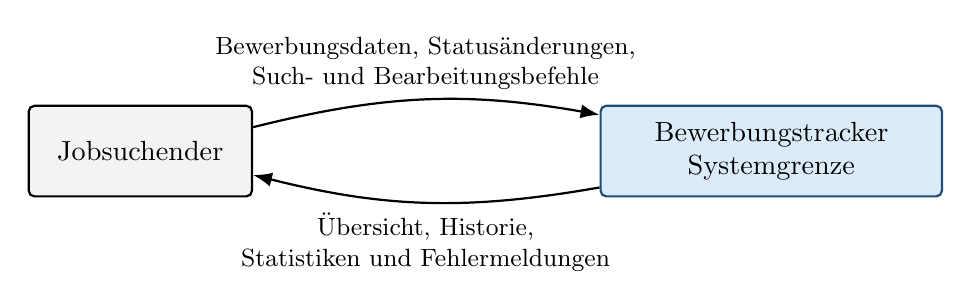
\begin{tikzpicture}[node distance=4.4cm]

  \node[actor] (user) {
    Jobsuchender
  };

  \node[
    system,
    right=of user,
    text width=4.1cm
  ] (system) {
    Bewerbungstracker\\
    Systemgrenze
  };

  \draw[
    connection,
    bend left=12
  ]
  (user) to
  node[
    above,
    align=center,
    font=\small
  ] {
    Bewerbungsdaten, Statusänderungen,\\
    Such- und Bearbeitungsbefehle
  }
  (system);

  \draw[
    connection,
    bend left=12
  ]
  (system) to
  node[
    below,
    align=center,
    font=\small
  ] {
    Übersicht, Historie,\\
    Statistiken und Fehlermeldungen
  }
  (user);

\end{tikzpicture}
\caption{Fachlicher Kontext des Bewerbungstrackers}
\label{fig:functional-context}
\end{figure}

\subsection{Technischer Kontext}

Der Nutzer greift über einen Webbrowser auf das React-Frontend zu.
Das Frontend kommuniziert über eine REST-Schnittstelle und JSON-Nachrichten mit dem Spring-Boot-Backend.
Das Backend verarbeitet die Anfragen und greift über JDBC auf PostgreSQL zu.
Die Datenbank speichert die Bewerbungen und die zugehörigen Historieneinträge.
Vorschlagsdaten für Unternehmen, Positionen und Standorte lädt das Frontend direkt aus statischen CSV-Dateien.
Weitere externe Dienste oder Schnittstellen werden nicht verwendet.

\vspace{0.5cm}
\begin{figure}[H]
\centering
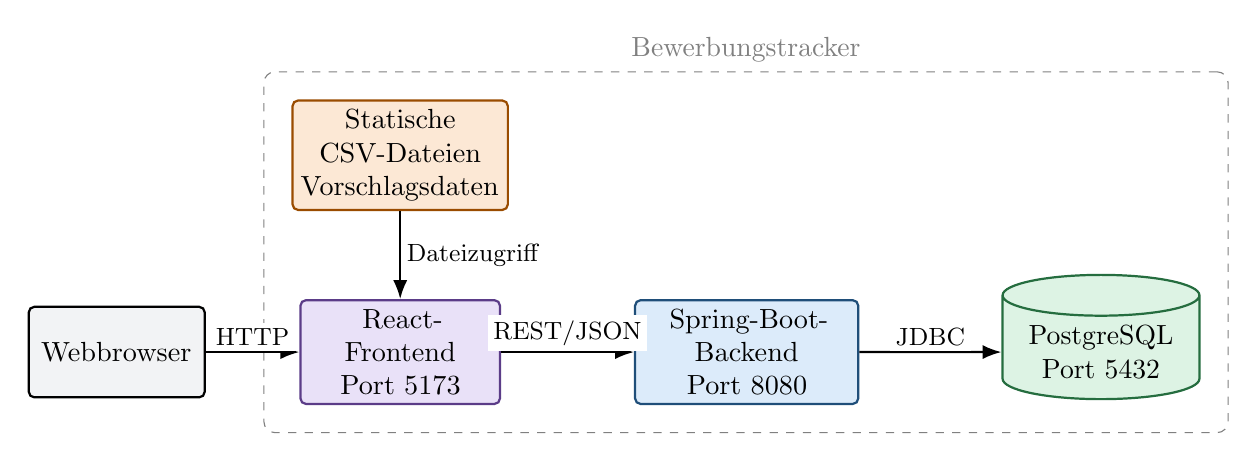
\begin{tikzpicture}

  \node[
    actor,
    text width=2cm
  ] (browser) at (0,0) {
    Webbrowser
  };

  \node[
    frontend,
    text width=2.3cm
  ] (frontend) at (3.6,0) {
    React-Frontend\\
    Port 5173
  };

  \node[
    backend,
    text width=2.6cm
  ] (backend) at (8,0) {
    Spring-Boot-Backend\\
    Port 8080
  };

  \node[
    database,
    minimum width=2.5cm
  ] (database) at (12.5,0) {
    PostgreSQL\\
    Port 5432
  };

  \node[
    filebox,
    text width=2.5cm
  ] (csv) at (3.6,2.5) {
    Statische CSV-Dateien\\
    Vorschlagsdaten
  };

  \draw[connection]
  (browser) --
  node[
    midway,
    above,
    fill=white,
    inner sep=2pt,
    font=\small
  ] {
    HTTP
  }
  (frontend);

  \draw[connection]
  (frontend) --
  node[
    midway,
    above,
    fill=white,
    inner sep=2pt,
    font=\small
  ] {
    REST/JSON
  }
  (backend);

  \draw[connection]
  (backend) --
  node[
    midway,
    above,
    fill=white,
    inner sep=2pt,
    font=\small
  ] {
    JDBC
  }
  (database);

  \draw[connection]
  (csv) --
  node[
    midway,
    right,
    fill=white,
    inner sep=2pt,
    font=\small
  ] {
    Dateizugriff
  }
  (frontend);

  \begin{scope}[on background layer]
    \node[
      draw=gray,
      dashed,
      rounded corners=4pt,
      fit=(frontend)(backend)(database)(csv),
      inner sep=0.35cm,
      label={
        [gray]above:Bewerbungstracker
      }
    ] {};
  \end{scope}

\end{tikzpicture}
\caption{Technischer Kontext des Bewerbungstrackers}
\label{fig:technical-context}
\end{figure}





% ============================  4 Lösungsstrategie ✓ =============================

\section{Lösungsstrategie}
\label{sec:solution-strategy}


% 4.1 - Layered Architecture
\subsection{Layered Architecture}

Die Layered Architecture gliedert das Backend in Schichten mit klar getrennten Verantwortlichkeiten.
In der umgesetzten geschlossenen Schichtenarchitektur darf jede Schicht nur auf die unmittelbar darunterliegende Schicht zugreifen \cite{richards2020}.

Das Backend besteht aus drei Schichten:

\begin{itemize}
  \item \textbf{Präsentationsschicht:} Verarbeitung von HTTP-Anfragen und Umwandlung der Request- und Response-Daten.
  \item \textbf{Geschäftslogikschicht:} Validierung von Eingaben, Prüfung der Statusregeln und Koordination fachlicher Abläufe.
  \item \textbf{Persistenzschicht:} Ausführung der SQL-Anweisungen und Abbildung der Datenbankeinträge auf Domänenobjekte.
\end{itemize}


% 4.2 - Umsetzung im Bewerbungstracker
\subsection{Umsetzung im Bewerbungstracker}

Das Backend ist als monolithische Spring-Boot-Anwendung umgesetzt.
Die drei Schichten sind in getrennten Paketen organisiert, werden jedoch gemeinsam gebaut und bereitgestellt.
Anfragen werden vom \texttt{ApplicationController} über den \texttt{ApplicationService} an das \texttt{ApplicationRepository} weitergegeben, ohne eine Schicht zu überspringen.
Das React-Frontend ist ein separater Client und kommuniziert über die REST-Schnittstelle mit dem Backend.

\vspace{0.5cm}

\begin{figure}[H]
\centering
\scalebox{0.9}{
  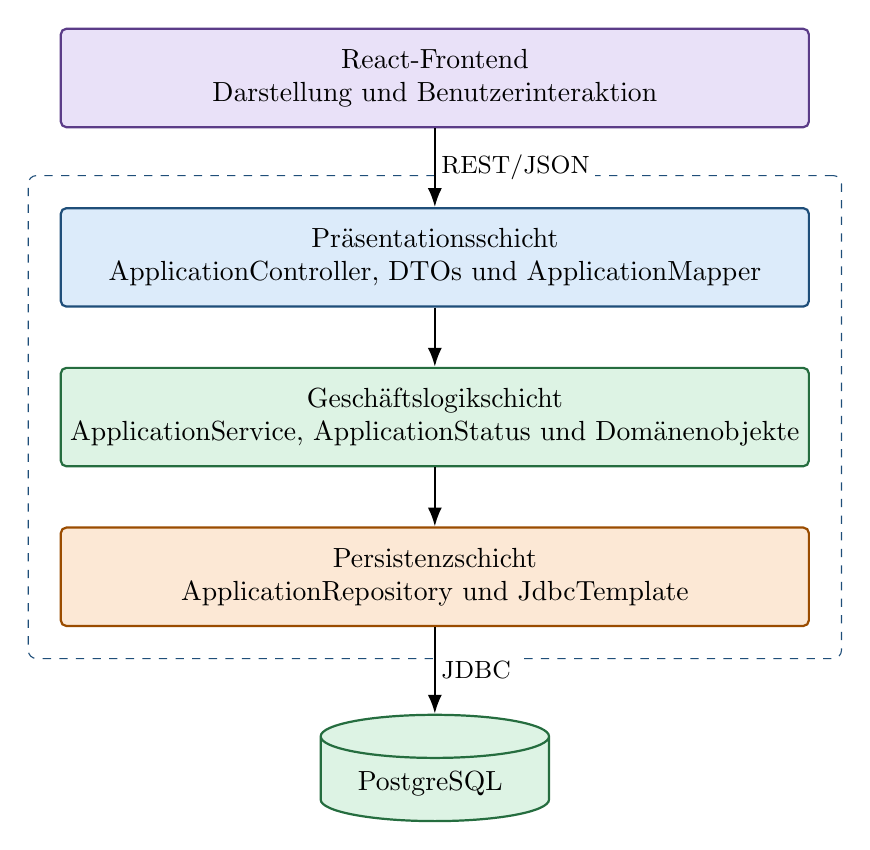
\begin{tikzpicture}[node distance=0.75cm]

  \node[
    layer,
    fill=LayerPurple,
    draw=DarkPurple
  ] (client) {
    React-Frontend\\
    Darstellung und Benutzerinteraktion
  };

  \node[
    layer,
    fill=LayerBlue,
    draw=DarkBlue,
    below=1cm of client
  ] (presentation) {
    Präsentationsschicht\\
    ApplicationController, DTOs und ApplicationMapper
  };

  \node[
    layer,
    fill=LayerGreen,
    draw=DarkGreen,
    below=of presentation
  ] (business) {
    Geschäftslogikschicht\\
    ApplicationService, ApplicationStatus und Domänenobjekte
  };

  \node[
    layer,
    fill=LayerOrange,
    draw=DarkOrange,
    below=of business
  ] (persistence) {
    Persistenzschicht\\
    ApplicationRepository und JdbcTemplate
  };

  \node[
    database,
    below=1.1cm of persistence
  ] (database) {
    PostgreSQL
  };

  \draw[connection]
  (client) --
  node[
    midway,
    right,
    fill=white,
    inner sep=2pt,
    font=\small
  ] {
    REST/JSON
  }
  (presentation);

  \draw[connection]
  (presentation) --
  (business);

  \draw[connection]
  (business) --
  (persistence);

  \draw[connection]
  (persistence) --
  node[
    midway,
    right,
    fill=white,
    inner sep=2pt,
    font=\small
  ] {
    JDBC
  }
  (database);

  \begin{scope}[on background layer]
    \node[
      draw=DarkBlue,
      dashed,
      rounded corners=3pt,
      fit=(presentation)(business)(persistence),
      inner sep=0.4cm
    ] {};
  \end{scope}

\end{tikzpicture}
}
\caption{Schichten und Abhängigkeitsrichtung des Bewerbungstrackers}
\label{fig:layers}
\end{figure}


% 4.3 - Eignung und Konsequenzen
\subsection{Eignung und Konsequenzen}

Die Layered Architecture wurde im Rahmen des Architekturprojekts als umzusetzender Architekturstil ausgewählt.
Bei der Übertragung auf den Bewerbungstracker ergeben sich sowohl Vorteile für die Strukturierung des Backends als auch Einschränkungen für dessen Weiterentwicklung.

\vspace{0.2cm}

\begin{table}[H]
\centering
\begin{tabularx}{\textwidth}{Y Y}
\toprule
\textbf{Vorteile für das Projekt} & \textbf{Nachteile und Konsequenzen} \\
\midrule

Klare Trennung der Verantwortlichkeiten &
Schichtübergreifende Funktionen erfordern Änderungen in mehreren Schichten. \\

Zentrale Umsetzung der Geschäftsregeln im \texttt{ApplicationService} &
Bei wachsendem Funktionsumfang kann der Service zu viele Verantwortlichkeiten übernehmen. \\

Nachvollziehbare Abhängigkeitsrichtung zwischen den Schichten &
Einfache Operationen werden teilweise ohne zusätzliche Verarbeitung durch mehrere Schichten weitergereicht. \\

Geringe Build- und Bereitstellungskomplexität des Backends &
Die Backend-Schichten können nicht unabhängig bereitgestellt werden. \\

\bottomrule
\end{tabularx}
\caption{Vorteile und Konsequenzen der umgesetzten Lösungsstrategie}
\label{tab:layered-tradeoffs}
\end{table}


% 4.4 - Technologie- und Betriebsstrategie
\subsection{Technologie- und Betriebsstrategie}

Frontend, Backend und Datenbank werden als getrennte Laufzeitkomponenten betrieben.
Die drei internen Backend-Schichten bleiben dagegen Bestandteil einer gemeinsamen Spring-Boot-Anwendung.

\vspace{0.2cm}

\begin{table}[H]
\centering
\begin{tabularx}{\textwidth}{L{2.7cm} L{3.8cm} Y}
\toprule
\textbf{Bereich} & \textbf{Technologie} & \textbf{Aufgabe im System} \\
\midrule

Frontend &
React, Vite und Bun &
Bereitstellung der browserbasierten Benutzeroberfläche. \\

Backend &
Java 21, Spring Boot und Maven &
REST-Schnittstelle, Geschäftslogik und Build des Backends. \\

Datenzugriff &
Spring JDBC &
Ausführung der SQL-Abfragen über \texttt{JdbcTemplate}. \\

Datenbank &
PostgreSQL 16 &
Speicherung der Bewerbungen und Historieneinträge. \\

Betrieb &
Docker Compose &
Gemeinsamer Start von Frontend, Backend und Datenbank. \\

\bottomrule
\end{tabularx}
\caption{Technologien und ihre Aufgaben im Bewerbungstracker}
\label{tab:technology-strategy}
\end{table}





% =============================  5 Bausteinsicht ✓ ===============================

\newpage
\section{Bausteinsicht}
\label{sec:building-block-view}

Die Bausteinsicht beschreibt die statische Zerlegung des Bewerbungstrackers.
Dabei wird zunächst das Gesamtsystem betrachtet und anschließend das Backend als zentraler Baustein weiter zerlegt.


% 5.1 - Ebene 1: Gesamtsystem
\subsection{Ebene 1: Gesamtsystem}

Das Gesamtsystem wird in Frontend, Backend, Datenbank und statische Vorschlagsdaten zerlegt.
Diese Zerlegung folgt den unterschiedlichen Verantwortlichkeiten für Benutzerinteraktion, Geschäftslogik und Datenhaltung.

\vspace{0.5cm}
\begin{figure}[H]
\centering
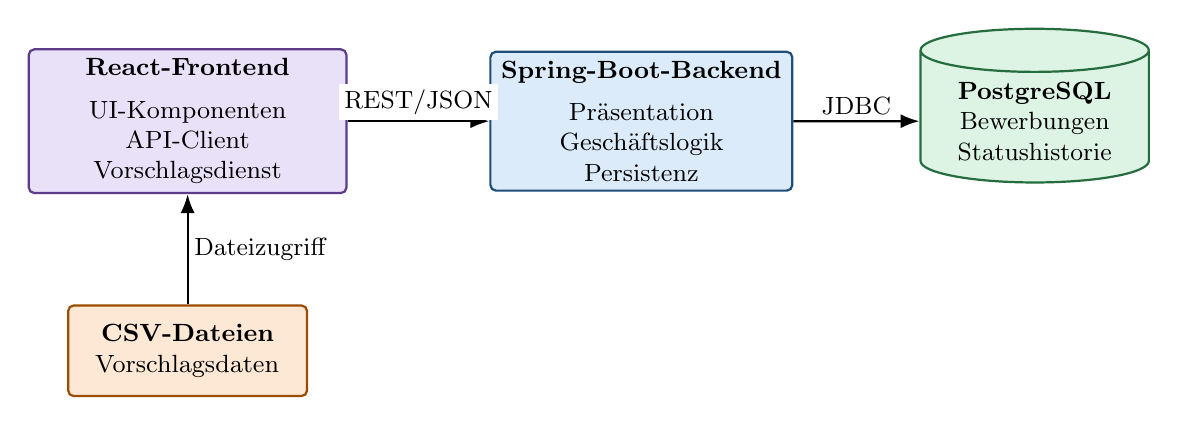
\begin{tikzpicture}[node distance=1.4cm and 1.8cm]

  \node[
    frontend,
    text width=3.8cm,
    font=\small
  ] (frontend) {
    \textbf{React-Frontend}\\[0.15cm]
    UI-Komponenten\\
    API-Client\\
    Vorschlagsdienst
  };

  \node[
    backend,
    right=of frontend,
    text width=3.6cm,
    font=\small
  ] (backend) {
    \textbf{Spring-Boot-Backend}\\[0.15cm]
    Präsentation\\
    Geschäftslogik\\
    Persistenz
  };

  \node[
    database,
    right=1.6cm of backend,
    font=\small
  ] (database) {
    \textbf{PostgreSQL}\\
    Bewerbungen\\
    Statushistorie
  };

  \node[
    filebox,
    below=1.4cm of frontend,
    font=\small
  ] (csv) {
    \textbf{CSV-Dateien}\\
    Vorschlagsdaten
  };

  \draw[connection]
  (frontend) --
  node[
    midway,
    above,
    fill=white,
    inner sep=2pt,
    font=\small
  ] {
    REST/JSON
  }
  (backend);

  \draw[connection]
  (backend) --
  node[
    midway,
    above,
    fill=white,
    inner sep=2pt,
    font=\small
  ] {
    JDBC
  }
  (database);

  \draw[connection]
  (csv) --
  node[
    midway,
    right,
    fill=white,
    inner sep=2pt,
    font=\small
  ] {
    Dateizugriff
  }
  (frontend);

\end{tikzpicture}
\caption{Bausteine des Gesamtsystems}
\label{fig:system-building-blocks}
\end{figure}

\textbf{React-Frontend.}
Das Frontend stellt die Benutzeroberfläche dar und verarbeitet die Eingaben des Nutzers.
Es verwaltet den lokalen Anwendungszustand, führt die Suche und Statistikberechnung aus und greift über REST auf das Backend zu.

\textbf{Spring-Boot-Backend.}
Das Backend verarbeitet die REST-Anfragen des Frontends.
Es führt die Geschäftsregeln aus und koordiniert den Zugriff auf die Datenbank.

\textbf{PostgreSQL.}
Die Datenbank speichert die Bewerbungen und die zugehörigen Historieneinträge dauerhaft.

\textbf{CSV-Vorschlagsdaten.}
Die statischen CSV-Dateien enthalten Vorschläge für Unternehmen, Positionen und Standorte.
Sie werden durch den Vorschlagsdienst des Frontends geladen und lokal ausgewertet.


% 5.2 - Ebene 2: Backend
\newpage
\subsection{Ebene 2: Backend}

Das Backend wird in Präsentationsschicht, Geschäftslogikschicht und Persistenzschicht zerlegt.
Die Abhängigkeiten zwischen den zentralen Bausteinen sind in Abbildung~\ref{fig:backend-building-blocks} dargestellt.

\vspace{0.5cm}
\begin{figure}[H]
\centering
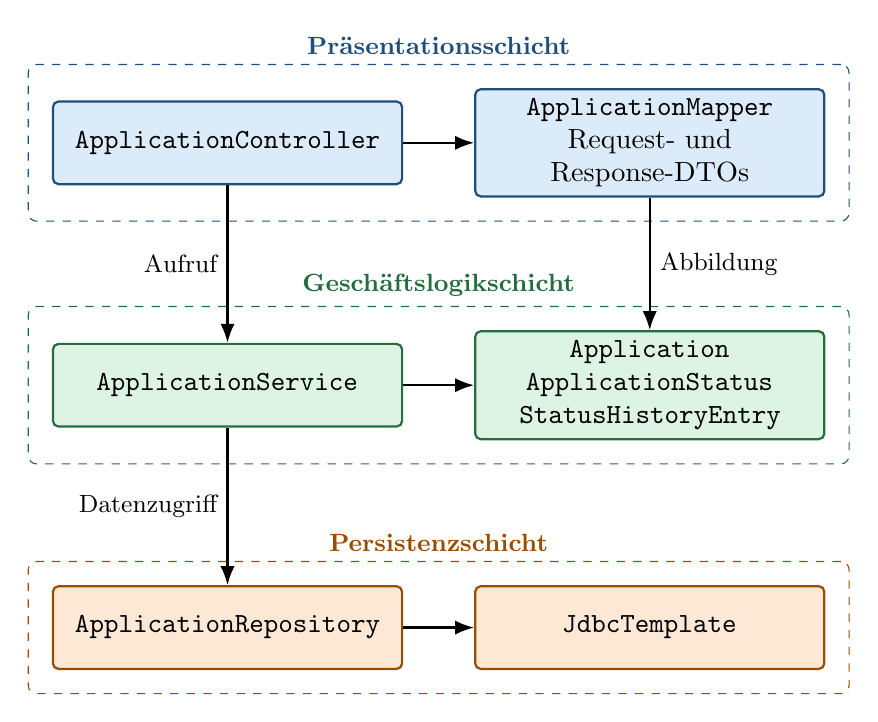
\begin{tikzpicture}[
  node distance=2cm and 0.9cm,
  component/.style={
    draw,
    rounded corners=2pt,
    thick,
    align=center,
    minimum height=1.05cm,
    text width=4.2cm
  }
]

  \node[
    component,
    fill=LayerBlue,
    draw=DarkBlue
  ] (controller) {
    \texttt{ApplicationController}
  };

  \node[
    component,
    fill=LayerBlue,
    draw=DarkBlue,
    right=of controller
  ] (presentationData) {
    \texttt{ApplicationMapper}\\
    Request- und Response-DTOs
  };

  \node[
    component,
    fill=LayerGreen,
    draw=DarkGreen,
    below=of controller
  ] (service) {
    \texttt{ApplicationService}
  };

  \node[
    component,
    fill=LayerGreen,
    draw=DarkGreen,
    right=of service
  ] (domain) {
    \texttt{Application}\\
    \texttt{ApplicationStatus}\\
    \texttt{StatusHistoryEntry}
  };

  \node[
    component,
    fill=LayerOrange,
    draw=DarkOrange,
    below=of service
  ] (repository) {
    \texttt{ApplicationRepository}
  };

  \node[
    component,
    fill=LayerOrange,
    draw=DarkOrange,
    right=of repository
  ] (jdbc) {
    \texttt{JdbcTemplate}
  };

  \draw[connection]
  (controller) --
  node[
    left,
    font=\small
  ] {
    Aufruf
  }
  (service);

  \draw[connection]
  (controller) --
  (presentationData);

  \draw[connection]
  (presentationData) --
  node[
    right,
    font=\small
  ] {
    Abbildung
  }
  (domain);

  \draw[connection]
  (service) --
  (domain);

  \draw[connection]
  (service) --
  node[
    left,
    font=\small
  ] {
    Datenzugriff
  }
  (repository);

  \draw[connection]
  (repository) --
  (jdbc);

  \begin{scope}[on background layer]

    \node[
      draw=DarkBlue,
      dashed,
      rounded corners=3pt,
      fit=(controller)(presentationData),
      inner sep=0.3cm,
      label={
        [font=\bfseries\small,text=DarkBlue]above:
        Präsentationsschicht
      }
    ] {};

    \node[
      draw=DarkGreen,
      dashed,
      rounded corners=3pt,
      fit=(service)(domain),
      inner sep=0.3cm,
      label={
        [font=\bfseries\small,text=DarkGreen]above:
        Geschäftslogikschicht
      }
    ] {};

    \node[
      draw=DarkOrange,
      dashed,
      rounded corners=3pt,
      fit=(repository)(jdbc),
      inner sep=0.3cm,
      label={
        [font=\bfseries\small,text=DarkOrange]above:
        Persistenzschicht
      }
    ] {};

  \end{scope}

\end{tikzpicture}
\caption{Wichtige Bausteine und Abhängigkeiten des Backends}
\label{fig:backend-building-blocks}
\end{figure}

\textbf{Präsentationsschicht.}
Der \texttt{ApplicationController} stellt die REST-Endpunkte bereit und delegiert eingehende Anfragen an den \texttt{ApplicationService}.
Der \texttt{ApplicationMapper} und die Request- und Response-DTOs übernehmen die Umwandlung der übertragenen Daten.

\textbf{Geschäftslogikschicht.}
Der \texttt{ApplicationService} führt die fachlichen Anwendungsfälle aus.
Die Domänenobjekte \texttt{Application} und \texttt{StatusHistoryEntry} bilden Bewerbungen und deren Historie ab.
Die Klasse \texttt{ApplicationStatus} definiert die zulässigen Statusübergänge.

\textbf{Persistenzschicht.}
Das \texttt{ApplicationRepository} lädt und speichert Bewerbungen und Historieneinträge.
Die SQL-Anweisungen werden über Spring JDBC und das \texttt{JdbcTemplate} ausgeführt.


% 5.3 - Schnittstelle zwischen Frontend und Backend
\newpage
\subsection{Schnittstelle zwischen Frontend und Backend}

Das Frontend greift ausschließlich über die REST-Schnittstelle auf das Backend zu. Request- und Response-Daten werden als JSON übertragen. 
Ungültige Eingaben führen zu \texttt{HTTP 400}, während unbekannte Bewerbungs-IDs mit \texttt{HTTP 404} beantwortet werden.

\vspace{0.5cm}
\begin{table}[H]
\centering
\small
\begin{tabularx}{\textwidth}{L{1.8cm} L{6.4cm} Y}
\toprule
\textbf{Methode} & \textbf{Pfad} & \textbf{Zweck} \\
\midrule

GET &
\path|/api/health| &
Erreichbarkeit des Backends prüfen. \\

GET &
\path|/api/applications| &
Alle Bewerbungen laden. \\

POST &
\path|/api/applications| &
Neue Bewerbung erstellen. \\

PUT &
\path|/api/applications/{id}| &
Bestehende Bewerbung bearbeiten. \\

PATCH &
\path|/api/applications/{id}/status| &
Zulässigen Statuswechsel durchführen. \\

POST &
\path|/api/applications/{id}/undo-last-status-change| &
Letzte Statusänderung zurücksetzen. \\

DELETE &
\path|/api/applications/{id}| &
Bewerbung löschen. \\

\bottomrule
\end{tabularx}
\caption{REST-Schnittstelle des Backends}
\label{tab:rest-endpoints}
\end{table}





% =============================  6 Laufzeitsicht ✓ ===============================

\section{Laufzeitsicht}
\label{sec:runtime-view}

Die Laufzeitsicht beschreibt das Zusammenspiel der Bausteine bei zentralen Anwendungsfällen.
Dargestellt werden das Laden und Erstellen von Bewerbungen sowie das Ändern und Zurücksetzen ihres Status.


% 6.1 - Laden der Bewerbungen
\subsection{Laden der Bewerbungen}

Beim Start der Anwendung werden die Bewerbungen in folgenden Schritten geladen:

\begin{enumerate}[leftmargin=1.6em,itemsep=0.3em]

  \item Das Frontend ruft zunächst \texttt{GET /api/health} auf und prüft die Erreichbarkeit des Backends.

  \item Nach erfolgreicher Prüfung fordert das Frontend über \texttt{GET /api/applications} alle Bewerbungen an.

  \item Der \texttt{ApplicationController} delegiert die Anfrage an den \texttt{ApplicationService}.

  \item Der Service ruft das \texttt{ApplicationRepository} auf.
  Das Repository lädt zunächst die Bewerbungen und anschließend für jede Bewerbung die zugehörigen Historieneinträge.

  \item Der \texttt{ApplicationMapper} wandelt die Domänenobjekte in Response-Objekte um.
  Der Controller gibt diese als JSON an das Frontend zurück.

  \item Das Frontend übernimmt die Bewerbungen in seinen lokalen Zustand.
  Bei einem Fehler wird der lokale Datenbestand geleert und das Backend als nicht erreichbar angezeigt.

\end{enumerate}


% 6.2 - Erstellen einer Bewerbung
\subsection{Erstellen einer Bewerbung}

Das Frontend übermittelt die eingegebenen Bewerbungsdaten mit einer POST-Anfrage an das Backend.
Abbildung~\ref{fig:runtime-create} zeigt die Verarbeitung der Anfrage durch die drei Backend-Schichten.

\vspace{0.4cm}

\begin{figure}[H]
\centering
\resizebox{\textwidth}{!}{
  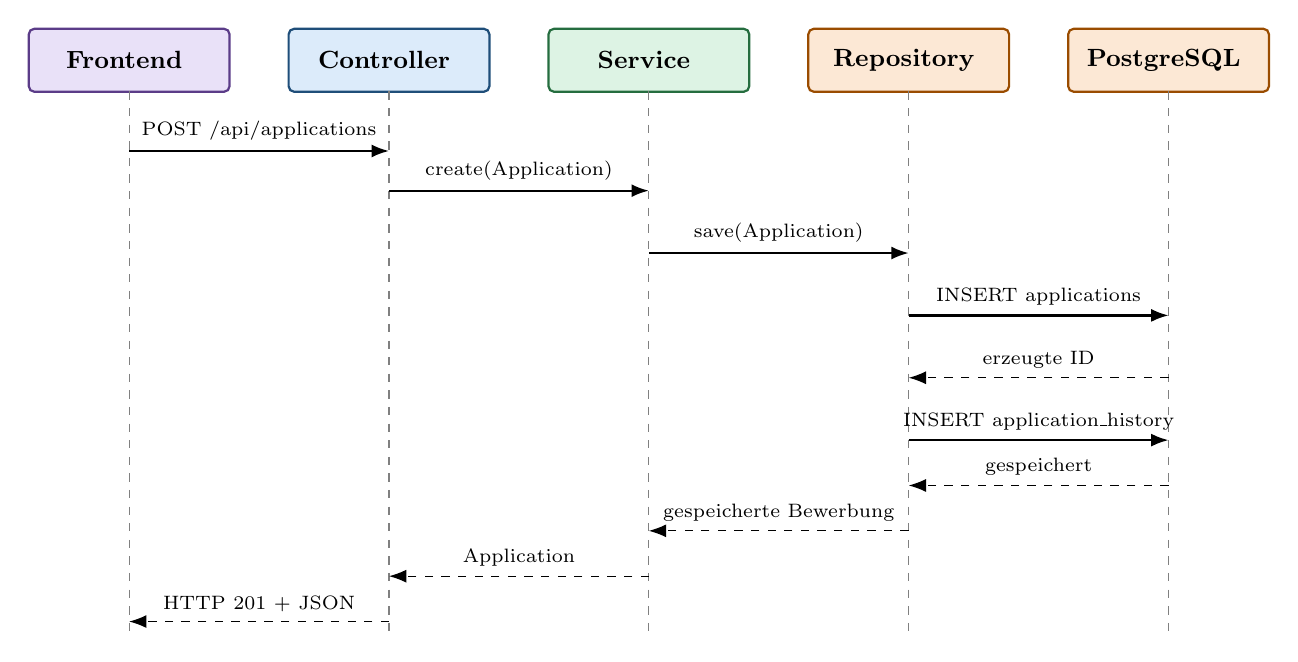
\begin{tikzpicture}[x=3.3cm,y=-0.72cm,font=\small]

  \node[
    participant,
    fill=LayerPurple,
    draw=DarkPurple,
    font=\bfseries\small
  ] at (0,0) (frontend) {
    Frontend
  };

  \node[
    participant,
    fill=LayerBlue,
    draw=DarkBlue,
    font=\bfseries\small
  ] at (1,0) (controller) {
    Controller
  };

  \node[
    participant,
    fill=LayerGreen,
    draw=DarkGreen,
    font=\bfseries\small
  ] at (2,0) (service) {
    Service
  };

  \node[
    participant,
    fill=LayerOrange,
    draw=DarkOrange,
    font=\bfseries\small
  ] at (3,0) (repository) {
    Repository
  };

  \node[
    participant,
    fill=LayerOrange,
    draw=DarkOrange,
    font=\bfseries\small
  ] at (4,0) (database) {
    PostgreSQL
  };

  \foreach \x in {0,1,2,3,4} {
    \draw[dashed,gray]
    (\x,0.55) --
    (\x,10.1);
  }

  \draw[message]
  (frontend.center |- 0,1.6) --
  node[
    above,
    font=\scriptsize
  ] {
    POST /api/applications
  }
  (controller.center |- 0,1.6);

  \draw[message]
  (controller.center |- 0,2.3) --
  node[
    above,
    font=\scriptsize
  ] {
    create(Application)
  }
  (service.center |- 0,2.3);

  \draw[message]
  (service.center |- 0,3.4) --
  node[
    above,
    font=\scriptsize
  ] {
    save(Application)
  }
  (repository.center |- 0,3.4);

  \draw[message]
  (repository.center |- 0,4.5) --
  node[
    above,
    font=\scriptsize
  ] {
    INSERT applications
  }
  (database.center |- 0,4.5);

  \draw[return]
  (database.center |- 0,5.6) --
  node[
    above,
    font=\scriptsize
  ] {
    erzeugte ID
  }
  (repository.center |- 0,5.6);

  \draw[message]
  (repository.center |- 0,6.7) --
  node[
    above,
    font=\scriptsize
  ] {
    INSERT application\_history
  }
  (database.center |- 0,6.7);

  \draw[return]
  (database.center |- 0,7.5) --
  node[
    above,
    font=\scriptsize
  ] {
    gespeichert
  }
  (repository.center |- 0,7.5);

  \draw[return]
  (repository.center |- 0,8.3) --
  node[
    above,
    font=\scriptsize
  ] {
    gespeicherte Bewerbung
  }
  (service.center |- 0,8.3);

  \draw[return]
  (service.center |- 0,9.1) --
  node[
    above,
    font=\scriptsize
  ] {
    Application
  }
  (controller.center |- 0,9.1);

  \draw[return]
  (controller.center |- 0,9.9) --
  node[
    above,
    font=\scriptsize
  ] {
    HTTP 201 + JSON
  }
  (frontend.center |- 0,9.9);

\end{tikzpicture}
}
\caption{Laufzeitablauf beim Erstellen einer Bewerbung}
\label{fig:runtime-create}
\end{figure}

Der \texttt{ApplicationService} normalisiert Firma, Position, Standort und Notizen.
Firma und Position sind Pflichtfelder.
Negative Gehaltswerte und ein Mindestgehalt oberhalb des Maximalgehalts werden abgelehnt.
Der initiale Status wird unabhängig von der Frontend-Eingabe auf \texttt{DRAFT} gesetzt.
Zusätzlich wird ein erster Historieneintrag für die Erstellung der Bewerbung erzeugt.

Bei einer ungültigen Eingabe wird die Verarbeitung vor dem Speichern abgebrochen.
Der Controller beantwortet die Anfrage in diesem Fall mit \texttt{HTTP 400}.


% 6.3 - Ändern und Zurücksetzen eines Status
\newpage
\subsection{Ändern und Zurücksetzen eines Status}

Bei einer Statusänderung sendet das Frontend den gewünschten Zielstatus an das Backend.
Abbildung~\ref{fig:runtime-status} zeigt den erfolgreichen Ablauf einer zulässigen Statusänderung.

\vspace{0.4cm}

\begin{figure}[H]
\centering
\resizebox{\textwidth}{!}{
  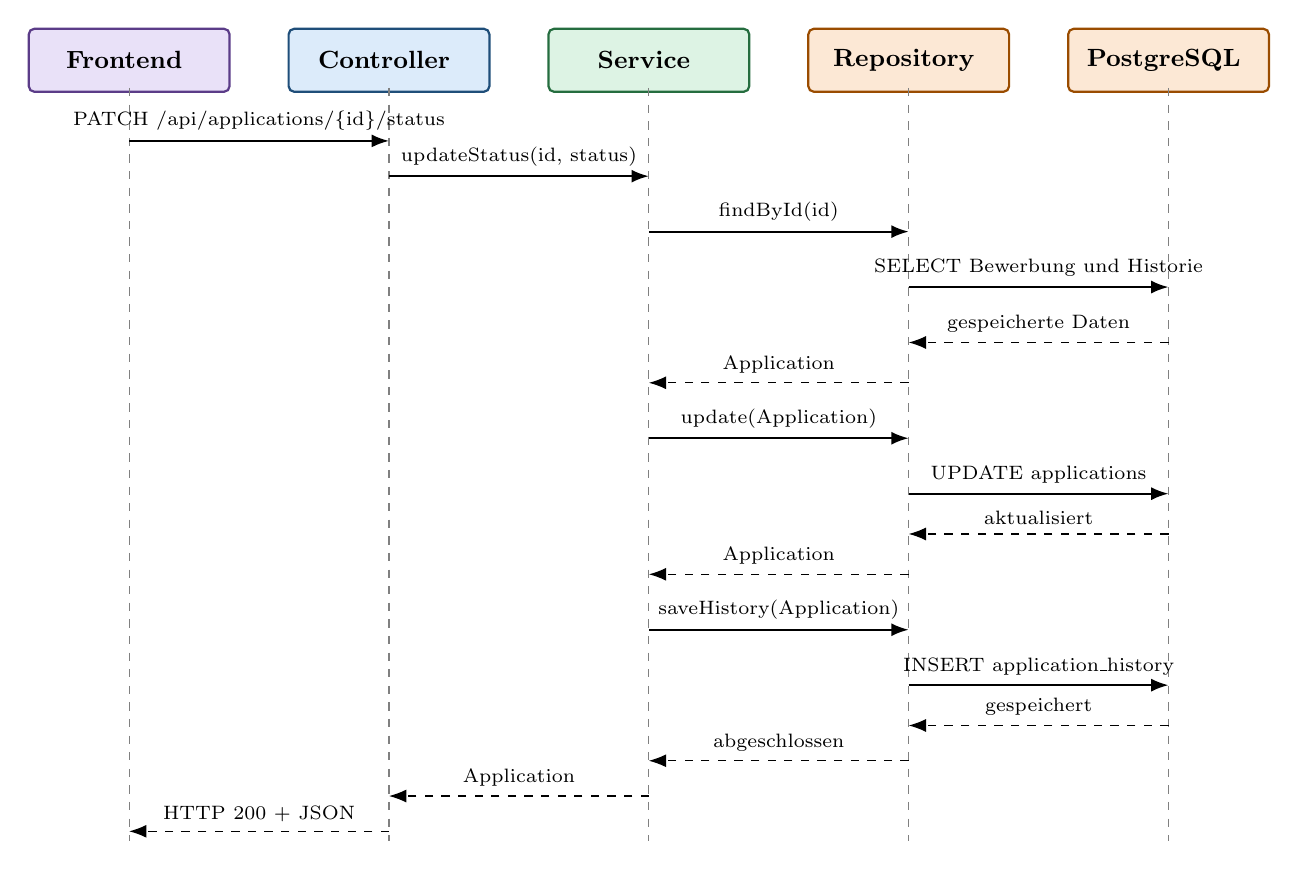
\begin{tikzpicture}[x=3.3cm,y=-0.64cm,font=\small]

  \node[
    participant,
    fill=LayerPurple,
    draw=DarkPurple,
    font=\bfseries\small
  ] at (0,0) (frontend) {
    Frontend
  };

  \node[
    participant,
    fill=LayerBlue,
    draw=DarkBlue,
    font=\bfseries\small
  ] at (1,0) (controller) {
    Controller
  };

  \node[
    participant,
    fill=LayerGreen,
    draw=DarkGreen,
    font=\bfseries\small
  ] at (2,0) (service) {
    Service
  };

  \node[
    participant,
    fill=LayerOrange,
    draw=DarkOrange,
    font=\bfseries\small
  ] at (3,0) (repository) {
    Repository
  };

  \node[
    participant,
    fill=LayerOrange,
    draw=DarkOrange,
    font=\bfseries\small
  ] at (4,0) (database) {
    PostgreSQL
  };

  \foreach \x in {0,1,2,3,4} {
    \draw[dashed,gray]
    (\x,0.55) --
    (\x,15.5);
  }

  \draw[message]
  (frontend.center |- 0,1.6) --
  node[
    above,
    font=\scriptsize
  ] {
    PATCH /api/applications/\{id\}/status
  }
  (controller.center |- 0,1.6);

  \draw[message]
  (controller.center |- 0,2.3) --
  node[
    above,
    font=\scriptsize
  ] {
    updateStatus(id, status)
  }
  (service.center |- 0,2.3);

  \draw[message]
  (service.center |- 0,3.4) --
  node[
    above,
    font=\scriptsize
  ] {
    findById(id)
  }
  (repository.center |- 0,3.4);

  \draw[message]
  (repository.center |- 0,4.5) --
  node[
    above,
    font=\scriptsize
  ] {
    SELECT Bewerbung und Historie
  }
  (database.center |- 0,4.5);

  \draw[return]
  (database.center |- 0,5.6) --
  node[
    above,
    font=\scriptsize
  ] {
    gespeicherte Daten
  }
  (repository.center |- 0,5.6);

  \draw[return]
  (repository.center |- 0,6.4) --
  node[
    above,
    font=\scriptsize
  ] {
    Application
  }
  (service.center |- 0,6.4);

  \draw[message]
  (service.center |- 0,7.5) --
  node[
    above,
    font=\scriptsize
  ] {
    update(Application)
  }
  (repository.center |- 0,7.5);

  \draw[message]
  (repository.center |- 0,8.6) --
  node[
    above,
    font=\scriptsize
  ] {
    UPDATE applications
  }
  (database.center |- 0,8.6);

  \draw[return]
  (database.center |- 0,9.4) --
  node[
    above,
    font=\scriptsize
  ] {
    aktualisiert
  }
  (repository.center |- 0,9.4);

  \draw[return]
  (repository.center |- 0,10.2) --
  node[
    above,
    font=\scriptsize
  ] {
    Application
  }
  (service.center |- 0,10.2);

  \draw[message]
  (service.center |- 0,11.3) --
  node[
    above,
    font=\scriptsize
  ] {
    saveHistory(Application)
  }
  (repository.center |- 0,11.3);

  \draw[message]
  (repository.center |- 0,12.4) --
  node[
    above,
    font=\scriptsize
  ] {
    INSERT application\_history
  }
  (database.center |- 0,12.4);

  \draw[return]
  (database.center |- 0,13.2) --
  node[
    above,
    font=\scriptsize
  ] {
    gespeichert
  }
  (repository.center |- 0,13.2);

  \draw[return]
  (repository.center |- 0,13.9) --
  node[
    above,
    font=\scriptsize
  ] {
    abgeschlossen
  }
  (service.center |- 0,13.9);

  \draw[return]
  (service.center |- 0,14.6) --
  node[
    above,
    font=\scriptsize
  ] {
    Application
  }
  (controller.center |- 0,14.6);

  \draw[return]
  (controller.center |- 0,15.3) --
  node[
    above,
    font=\scriptsize
  ] {
    HTTP 200 + JSON
  }
  (frontend.center |- 0,15.3);

\end{tikzpicture}
}
\caption{Laufzeitablauf bei einer Statusänderung}
\label{fig:runtime-status}
\end{figure}

Das Frontend verhindert bekannte unzulässige Übergänge bereits in der Benutzeroberfläche.
Die verbindliche Prüfung erfolgt im Backend anhand der Regeln in \texttt{ApplicationStatus}.
Bei einem unzulässigen Übergang wird keine Änderung gespeichert.
Der Controller beantwortet die Anfrage in diesem Fall mit \texttt{HTTP 400}.

Beim Zurücksetzen ermittelt der Service den letzten wirksamen Statuswechsel.
Der aktuelle Status wird auf den vorherigen Status gesetzt.
Zusätzlich wird ein Historieneintrag vom Typ \texttt{STATUS\_CHANGE\_UNDONE} erzeugt.
Die Bewerbung und der neue Historieneintrag werden nacheinander über das Repository gespeichert.





% ===========================  7 Verteilungssicht  ==============================

\newpage
\section{Verteilungssicht}
\label{sec:deployment-view}

Die Anwendung wird lokal über Docker Compose auf drei Container verteilt.
Der Frontend-Container stellt die React-Anwendung bereit, der Backend-Container führt die Geschäftslogik aus und der PostgreSQL-Container übernimmt die Datenhaltung.
Alle Container befinden sich in einem gemeinsamen Docker-Netzwerk.

Der Browser lädt das Frontend über Port~5173.
Die anschließend im Browser ausgeführte React-Anwendung greift über Port~8080 auf die REST-Schnittstelle des Backends zu.
Das Backend verbindet sich innerhalb des Docker-Netzwerks über \texttt{postgres:5432} mit der Datenbank.

\vspace{0.4cm}

\begin{figure}[H]
\centering
\resizebox{\textwidth}{!}{
  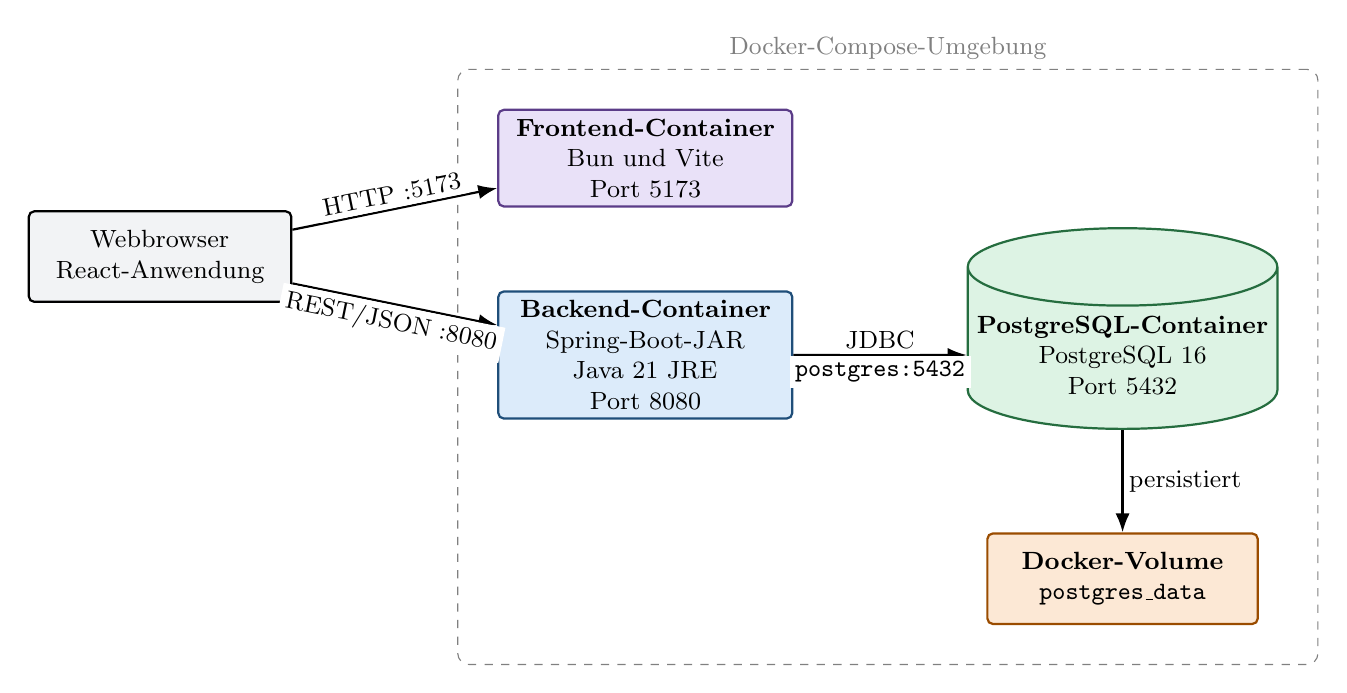
\begin{tikzpicture}[
  node distance=1.2cm and 2.2cm,
  font=\small
]

  \node[
    actor,
    text width=3.1cm
  ] (browser) {
    Webbrowser\\
    React-Anwendung
  };

  \node[
    frontend,
    right=2.6cm of browser,
    yshift=1.25cm,
    text width=3.5cm
  ] (frontend) {
    \textbf{Frontend-Container}\\
    Bun und Vite\\
    Port 5173
  };

  \node[
    backend,
    right=2.6cm of browser,
    yshift=-1.25cm,
    text width=3.5cm
  ] (backend) {
    \textbf{Backend-Container}\\
    Spring-Boot-JAR\\
    Java 21 JRE\\
    Port 8080
  };

  \node[
    database,
    right=2.2cm of backend,
    minimum width=3.5cm,
    minimum height=1.8cm
  ] (postgres) {
    \textbf{PostgreSQL-Container}\\
    PostgreSQL 16\\
    Port 5432
  };

  \node[
    filebox,
    below=1.3cm of postgres,
    text width=3.2cm
  ] (volume) {
    \textbf{Docker-Volume}\\
    \texttt{postgres\_data}
  };

  \draw[connection]
  (browser) --
  node[
    above,
    sloped,
    fill=white,
    inner sep=2pt
  ] {
    HTTP :5173
  }
  (frontend);

  \draw[connection]
  (browser) --
  node[
    below,
    sloped,
    fill=white,
    inner sep=2pt
  ] {
    REST/JSON :8080
  }
  (backend);

  \draw[connection]
  (backend) --
  node[
    above,
    fill=white,
    inner sep=2pt
  ] {
    JDBC
  }
  node[
    below,
    fill=white,
    inner sep=2pt
  ] {
    \texttt{postgres:5432}
  }
  (postgres);

  \draw[connection]
  (postgres) --
  node[
    right,
    fill=white,
    inner sep=2pt
  ] {
    persistiert
  }
  (volume);

  \begin{scope}[on background layer]
    \node[
      draw=gray,
      dashed,
      rounded corners=4pt,
      fit=(frontend)(backend)(postgres)(volume),
      inner sep=0.5cm,
      label={
        [gray]above:Docker-Compose-Umgebung
      }
    ] {};
  \end{scope}

\end{tikzpicture}
}
\caption{Lokale Verteilung des Bewerbungstrackers}
\label{fig:deployment}
\end{figure}

Der Backend-Container ist vom PostgreSQL-Container abhängig.
Er wird erst gestartet, nachdem der mit \texttt{pg\_isready} ausgeführte Datenbank-Healthcheck erfolgreich war.
Der Frontend-Container besitzt ebenfalls eine Startabhängigkeit zum Backend, wartet jedoch nicht auf dessen vollständige Betriebsbereitschaft.
Das Frontend prüft die Erreichbarkeit deshalb zusätzlich über den Endpunkt \texttt{/api/health}.

Die Backend-Adresse des Frontends kann über \texttt{VITE\_API\_BASE\_URL} konfiguriert werden.
Ohne eine abweichende Konfiguration verwendet das Frontend \texttt{http://localhost:8080}.
Das Backend erhält die Datenbankadresse und die Zugangsdaten über Spring-Umgebungsvariablen.

Die Datenbankdateien werden im Docker-Volume \texttt{postgres\_data} gespeichert und bleiben dadurch nach einem Neustart der Container erhalten.
PostgreSQL ist zusätzlich über Port~5432 des Hosts für Entwicklungszugriffe erreichbar.
Die verwendeten Zugangsdaten und veröffentlichten Ports sind für die lokale Entwicklungsumgebung vorgesehen und stellen keine produktive Sicherheitskonfiguration dar.




% ======================  8 Querschnittliche Konzepte  ==========================

\newpage
\section{Querschnittliche Konzepte}
\label{sec:crosscutting-concepts}


% 8.1 - Statusmodell und Validierung
\subsection{Statusmodell und Validierung}

Die Statuspipeline bildet die zentrale fachliche Regel des Bewerbungstrackers.
Die zulässigen Übergänge sind im Backend in \texttt{ApplicationStatus} definiert.
Das Frontend spiegelt diese Regeln, um unzulässige Benutzeraktionen bereits in der Oberfläche zu verhindern.
Die verbindliche Prüfung erfolgt jedoch immer in der Geschäftslogikschicht.

\vspace{0.3cm}

\begin{figure}[H]
\centering
\resizebox{\textwidth}{!}{
  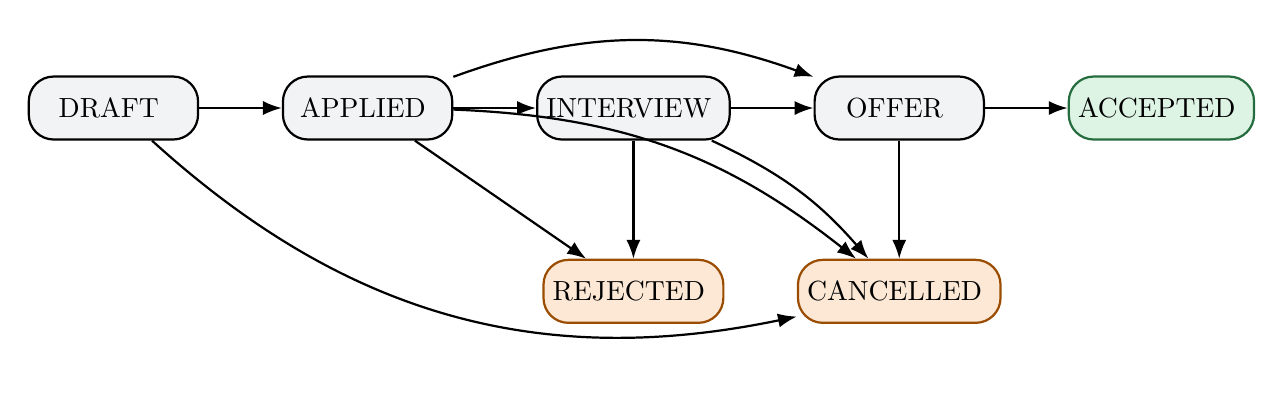
\begin{tikzpicture}[
  node distance=1.25cm and 1.05cm
]

  \node[
    state
  ] (draft) {
    DRAFT
  };

  \node[
    state,
    right=of draft
  ] (applied) {
    APPLIED
  };

  \node[
    state,
    right=of applied
  ] (interview) {
    INTERVIEW
  };

  \node[
    state,
    right=of interview
  ] (offer) {
    OFFER
  };

  \node[
    state,
    right=of offer,
    fill=LayerGreen,
    draw=DarkGreen
  ] (accepted) {
    ACCEPTED
  };

  \node[
    state,
    below=1.5cm of interview,
    fill=LayerOrange,
    draw=DarkOrange
  ] (rejected) {
    REJECTED
  };

  \node[
    state,
    below=1.5cm of offer,
    fill=LayerOrange,
    draw=DarkOrange
  ] (cancelled) {
    CANCELLED
  };

  \draw[connection]
  (draft) --
  (applied);

  \draw[connection]
  (applied) --
  (interview);

  \draw[connection]
  (interview) --
  (offer);

  \draw[connection]
  (offer) --
  (accepted);

  \draw[connection]
  (applied) --
  (rejected);

  \draw[connection]
  (interview) --
  (rejected);

  \draw[connection]
  (offer) --
  (cancelled);

  \draw[
    connection,
    bend right=27
  ]
  (draft) to
  (cancelled);

  \draw[
    connection,
    bend left=20
  ]
  (applied) to
  (offer);

  \draw[
    connection,
    bend left=18
  ]
  (applied) to
  (cancelled);

  \draw[
    connection,
    bend left=12
  ]
  (interview) to
  (cancelled);

\end{tikzpicture}
}
\caption{Zulässige Statusübergänge}
\label{fig:status-model}
\end{figure}

Beim Erstellen einer Bewerbung sind Firma und Position verpflichtend.
Gehaltswerte dürfen nicht negativ sein.
Bei einem Gehaltsbereich darf das Mindestgehalt nicht über dem Maximalgehalt liegen.
Der initiale Status wird unabhängig von den übertragenen Daten auf \texttt{DRAFT} gesetzt.

Inhaltliche Änderungen und Statusänderungen werden über getrennte REST-Endpunkte verarbeitet.
Dadurch können Statuswechsel unabhängig von Änderungen der übrigen Bewerbungsdaten validiert und protokolliert werden.


% 8.2 - Fehlerbehandlung
\subsection{Fehlerbehandlung}

Fachliche Fehler werden auf HTTP-Statuscodes abgebildet.
Verbindungsfehler behandelt das Frontend selbst.

\begin{table}[H]
\centering
\small
\begin{tabularx}{\textwidth}{L{3.5cm} L{2.2cm} Y}
\toprule
\textbf{Situation} & \textbf{Status} & \textbf{Reaktion} \\
\midrule

Ungültige Eingabe oder Statuswechsel &
400 &
JSON-Antwort mit fachlicher Fehlermeldung. \\

Unbekannte Bewerbungs-ID &
404 &
Die \texttt{ApplicationNotFoundException} wird in eine JSON-Fehlerantwort übersetzt. \\

Erfolgreiches Löschen &
204 &
Antwort ohne Response-Body. \\

Backend nicht erreichbar &
-- &
Lokale Daten werden geleert und das Backend als nicht erreichbar angezeigt. \\

\bottomrule
\end{tabularx}
\caption{Fehlerbehandlung in Frontend und Backend}
\label{tab:error-handling}
\end{table}


% 8.3 - Datenmodell, Persistenz und Änderungshistorie
\newpage
\subsection{Datenmodell, Persistenz und Änderungshistorie}

Die Tabelle \texttt{applications} speichert die Bewerbungsdaten und den aktuellen Status.
Die zugehörigen Änderungen werden in \texttt{application\_history} über eine 1:n-Beziehung protokolliert.

\vspace{0.3cm}

\begin{figure}[H]
\centering
\resizebox{0.9\textwidth}{!}{
  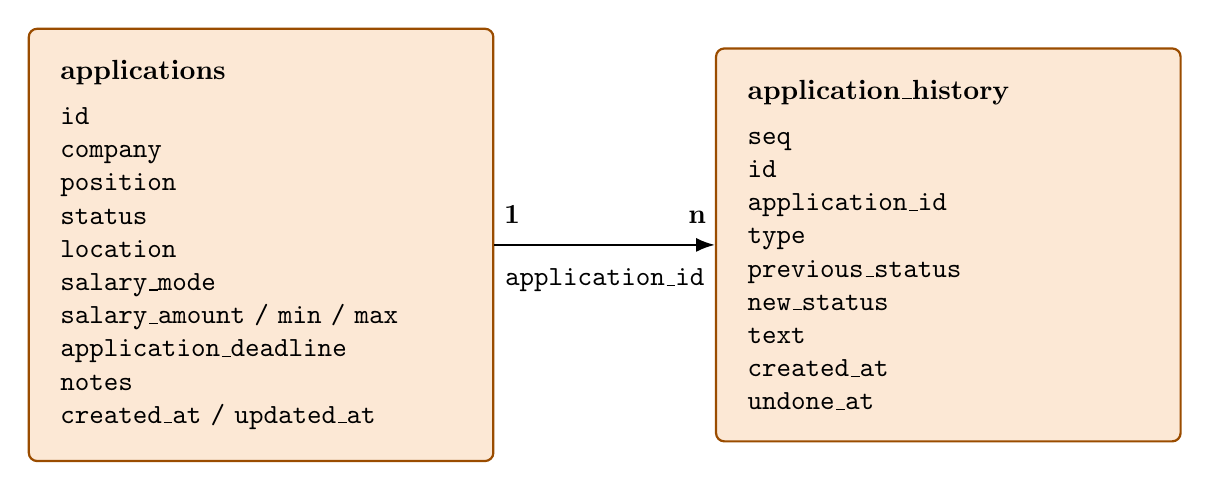
\begin{tikzpicture}[
  node distance=2.8cm
]

  \node[
    draw=DarkOrange,
    fill=LayerOrange,
    rounded corners=3pt,
    thick,
    align=left,
    text width=5.1cm,
    inner sep=0.4cm
  ] (applications) {
    \textbf{applications}\\[0.15cm]
    \texttt{id}\\
    \texttt{company}\\
    \texttt{position}\\
    \texttt{status}\\
    \texttt{location}\\
    \texttt{salary\_mode}\\
    \texttt{salary\_amount / min / max}\\
    \texttt{application\_deadline}\\
    \texttt{notes}\\
    \texttt{created\_at / updated\_at}
  };

  \node[
    draw=DarkOrange,
    fill=LayerOrange,
    rounded corners=3pt,
    thick,
    align=left,
    text width=5.1cm,
    inner sep=0.4cm,
    right=2.8cm of applications
  ] (history) {
    \textbf{application\_history}\\[0.15cm]
    \texttt{seq}\\
    \texttt{id}\\
    \texttt{application\_id}\\
    \texttt{type}\\
    \texttt{previous\_status}\\
    \texttt{new\_status}\\
    \texttt{text}\\
    \texttt{created\_at}\\
    \texttt{undone\_at}
  };

  \draw[connection]
  (applications.east) --
  node[
    pos=0.08,
    above=4pt,
    font=\bfseries
  ] {
    1
  }
  node[
    midway,
    below=5pt
  ] {
    \texttt{application\_id}
  }
  node[
    pos=0.92,
    above=4pt,
    font=\bfseries
  ] {
    n
  }
  (history.west);

\end{tikzpicture}
}
\caption{Vereinfachtes Datenmodell des Bewerbungstrackers}
\label{fig:data-model}
\end{figure}

Historieneinträge enthalten den Änderungstyp, den vorherigen und neuen Status, eine Beschreibung und den Erstellungszeitpunkt.
Verwendet werden die Typen \texttt{APPLICATION\_CREATED}, \texttt{STATUS\_CHANGED} und \texttt{STATUS\_CHANGE\_UNDONE}.

Die Persistenzschicht führt parametrisierte SQL-Anweisungen über \texttt{JdbcTemplate} aus.
Bewerbung und Historieneintrag werden dabei in getrennten Datenbankoperationen ohne gemeinsame Transaktion gespeichert.
Bei einem Fehler zwischen diesen Operationen kann deshalb ein inkonsistenter Zustand entstehen.


% 8.4 - Kommunikation und Sicherheit
\subsection{Kommunikation und Sicherheit}

Die Kommunikation zwischen Frontend und Backend erfolgt synchron über HTTP und JSON.
Nach dem Erstellen, Bearbeiten, Ändern oder Zurücksetzen eines Status übernimmt das Frontend die zurückgegebene Bewerbung in seinen lokalen Zustand.
Beim Löschen entfernt es den Eintrag nach einer erfolgreichen Antwort ohne Response-Body.

CORS erlaubt Browserzugriffe von \texttt{http://localhost:5173} und \texttt{http://localhost:5174}.
Andere Browser-Ursprünge werden nicht freigegeben.
CORS stellt jedoch keine Authentifizierung oder Zugriffskontrolle dar.

Der Bewerbungstracker ist als lokale Einzelbenutzer-Anwendung ausgelegt.
Eine Authentifizierung, Autorisierung und Trennung unterschiedlicher Benutzer war für diesen Anwendungsfall daher nicht erforderlich.
Jeder Client mit direktem Zugriff auf das Backend kann sämtliche Bewerbungen lesen und verändern.
Bei einer Bereitstellung außerhalb der lokalen Entwicklungsumgebung müsste ein entsprechender Zugriffsschutz ergänzt werden.





% ======================  9 Architekturentscheidungen  ==========================

\newpage
\section{Architekturentscheidungen}
\label{sec:architecture-decisions}

Die Layered Architecture war der im Architekturprojekt umzusetzende Architekturstil.
Dokumentiert werden daher die Entscheidungen zu ihrer konkreten Umsetzung im Bewerbungstracker.


% ADR-001
\subsection{ADR-001: Geschlossene Schichtenarchitektur}

\textbf{Kontext.}
Für das Backend musste eine konkrete Aufteilung der Verantwortlichkeiten festgelegt werden.
\textbf{Entscheidung.}
Das Backend besteht aus Präsentations-, Geschäftslogik- und Persistenzschicht.
Jede Schicht greift nur auf die unmittelbar darunterliegende Schicht zu.
\textbf{Konsequenz.}
Die Abhängigkeiten bleiben nachvollziehbar, während schichtübergreifende Funktionen Änderungen in mehreren Paketen erfordern können.


% ADR-002
\subsection{ADR-002: Getrenntes Frontend mit REST-Schnittstelle}

\textbf{Kontext.}
Benutzeroberfläche und Backend sollen getrennt strukturiert werden.
\textbf{Entscheidung.}
Das React-Frontend kommuniziert als separater Client über REST und JSON mit dem Spring-Boot-Backend.
\textbf{Konsequenz.}
Beide Teile können unabhängig entwickelt werden, benötigen aber eine klar definierte Schnittstelle und CORS-Konfiguration.


% ADR-003
\subsection{ADR-003: Relationale Persistenz mit Spring JDBC}

\textbf{Kontext.}
Bewerbungen und Statusänderungen müssen dauerhaft gespeichert werden.
\textbf{Entscheidung.}
Die Anwendung verwendet PostgreSQL und explizite SQL-Anweisungen über Spring JDBC.
\textbf{Konsequenz.}
SQL-Abfragen bleiben nachvollziehbar, während Mapping und Transaktionen selbst umgesetzt werden müssen.


% ADR-004
\subsection{ADR-004: Lokaler Betrieb mit Docker Compose}

\textbf{Kontext.}
Die drei Laufzeitkomponenten sollen gemeinsam und reproduzierbar gestartet werden.
\textbf{Entscheidung.}
Frontend, Backend und Datenbank werden als getrennte Container betrieben.
PostgreSQL verwendet ein persistentes Docker-Volume.
\textbf{Konsequenz.}
Der lokale Start wird vereinheitlicht, die Konfiguration ist jedoch nicht für einen produktiven Betrieb ausgelegt.





% =================  10 Risiken und technische Schulden  =======================

\newpage
\section{Risiken und technische Schulden}
\label{sec:risks}

Die aktuelle Implementierung erfüllt die Anforderungen des lokalen Lehrveranstaltungsprototyps.
Aus der vereinfachten Umsetzung ergeben sich jedoch Einschränkungen hinsichtlich Datenkonsistenz, Wartbarkeit, Skalierbarkeit und Betrieb.
Die folgende Tabelle beschreibt die erkannten Risiken und mögliche Maßnahmen für eine Weiterentwicklung.

\vspace{0.3cm}

\begin{table}[H]
\centering
\small
\renewcommand{\arraystretch}{1.2}
\begin{tabularx}{\textwidth}{L{3.5cm} Y Y}
\toprule
\textbf{Risiko oder Schuld} & \textbf{Auswirkung} & \textbf{Mögliche Maßnahme} \\
\midrule

Fehlende Transaktionsgrenzen &
Bewerbung und Historieneintrag können bei einem Teilfehler unterschiedliche Zustände aufweisen. &
Schreibende Service-Methoden mit \texttt{@Transactional} ausführen. \\

\addlinespace[0.15cm]

Undo-Persistenz &
Der Rücksetzzeitpunkt des ursprünglichen Historieneintrags wird nicht dauerhaft aktualisiert. &
Repository-Methode zum Aktualisieren von \texttt{undone\_at} ergänzen und testen. \\

\addlinespace[0.15cm]

Doppelte Statusregeln &
Frontend- und Backend-Regeln können bei Änderungen auseinanderlaufen. &
Statusregeln ausschließlich im Backend verwalten oder über die API bereitstellen. \\

\addlinespace[0.15cm]

N+1-Abfragen &
Für jede geladene Bewerbung wird eine zusätzliche Historienabfrage ausgeführt. &
Bewerbungen und Historieneinträge gemeinsam laden und im Repository gruppieren. \\

\addlinespace[0.15cm]

Fehlender Zugriffsschutz &
Bei einer externen Bereitstellung könnten alle Clients auf den gemeinsamen Datenbestand zugreifen. &
Bei einer Weiterentwicklung Authentifizierung und Besitzerzuordnung ergänzen. \\

\addlinespace[0.15cm]

Nur lokale Betriebskonfiguration &
Festgelegte Zugangsdaten, CORS-Adressen und der Vite-Entwicklungsserver sind nicht für einen produktiven Betrieb geeignet. &
Umgebungsabhängige Konfiguration, Secret-Verwaltung und einen Frontend-Produktions-Build einsetzen. \\

\addlinespace[0.15cm]

Begrenzte automatisierte Absicherung &
Fehler in Statusregeln, Undo-Funktion und Persistenz können unentdeckt bleiben. &
Unit- und Integrationstests für Service, Repository und REST-Endpunkte ergänzen. \\

\bottomrule
\end{tabularx}
\caption{Risiken und technische Schulden des Bewerbungstrackers}
\label{tab:risks}
\end{table}

\vspace{0.3cm}

Die Risiken sind für einen lokalen Lehrveranstaltungsprototyp vertretbar, begrenzen jedoch die Eignung für einen produktiven Betrieb.
Insbesondere die fehlenden Transaktionsgrenzen und die fehlerhafte Undo-Persistenz sollten vor einer Weiterverwendung korrigiert werden.

\clearpage





% ===========================  Literaturverzeichnis  =============================

\addcontentsline{toc}{section}{Literaturverzeichnis}
\begin{thebibliography}{9}

\bibitem{richards2020}
Mark Richards und Neal Ford:
\textit{Handbuch moderner Softwarearchitektur}.
O'Reilly Media, 2020.

\bibitem{arc42}
Peter Hruschka, Gernot Starke und Mitwirkende:
\textit{arc42 -- Template zur Dokumentation von Software- und Systemarchitekturen}.
\url{https://arc42.org/}, abgerufen am 31. Juli 2026.

\end{thebibliography}

\end{document}
